% Options for packages loaded elsewhere
\PassOptionsToPackage{unicode}{hyperref}
\PassOptionsToPackage{hyphens}{url}
\documentclass[
]{article}
\usepackage{xcolor}
\usepackage{amsmath,amssymb}
\setcounter{secnumdepth}{-\maxdimen} % remove section numbering
\usepackage{iftex}
\ifPDFTeX
  \usepackage[T1]{fontenc}
  \usepackage[utf8]{inputenc}
  \usepackage{textcomp} % provide euro and other symbols
\else % if luatex or xetex
  \usepackage{unicode-math} % this also loads fontspec
  \defaultfontfeatures{Scale=MatchLowercase}
  \defaultfontfeatures[\rmfamily]{Ligatures=TeX,Scale=1}
\fi
\usepackage{lmodern}
\ifPDFTeX\else
  % xetex/luatex font selection
\fi
% Use upquote if available, for straight quotes in verbatim environments
\IfFileExists{upquote.sty}{\usepackage{upquote}}{}
\IfFileExists{microtype.sty}{% use microtype if available
  \usepackage[]{microtype}
  \UseMicrotypeSet[protrusion]{basicmath} % disable protrusion for tt fonts
}{}
\makeatletter
\@ifundefined{KOMAClassName}{% if non-KOMA class
  \IfFileExists{parskip.sty}{%
    \usepackage{parskip}
  }{% else
    \setlength{\parindent}{0pt}
    \setlength{\parskip}{6pt plus 2pt minus 1pt}}
}{% if KOMA class
  \KOMAoptions{parskip=half}}
\makeatother
\usepackage{longtable,booktabs,array}
\usepackage{caption}
\captionsetup[table]{skip=6pt}
\newcounter{none} % for unnumbered tables
\usepackage{calc} % for calculating minipage widths
% Correct order of tables after \paragraph or \subparagraph
\usepackage{etoolbox}
\makeatletter
\patchcmd\longtable{\par}{\if@noskipsec\mbox{}\fi\par}{}{}
\makeatother
\usepackage{graphicx}
\makeatletter
\newsavebox\pandoc@box
\newcommand*\pandocbounded[1]{% scales image to fit in text height/width
  \sbox\pandoc@box{#1}%
  \Gscale@div\@tempa{\textheight}{\dimexpr\ht\pandoc@box+\dp\pandoc@box\relax}%
  \Gscale@div\@tempb{\linewidth}{\wd\pandoc@box}%
  \ifdim\@tempb\p@<\@tempa\p@\let\@tempa\@tempb\fi% select the smaller of both
  \ifdim\@tempa\p@<\p@\scalebox{\@tempa}{\usebox\pandoc@box}%
  \else\usebox{\pandoc@box}%
  \fi%
}
% Set default figure placement to htbp
\def\fps@figure{htbp}
\makeatother
% definitions for citeproc citations
\NewDocumentCommand\citeproctext{}{}
\NewDocumentCommand\citeproc{mm}{%
  \begingroup\def\citeproctext{#2}\cite{#1}\endgroup}
\makeatletter
 % allow citations to break across lines
 \let\@cite@ofmt\@firstofone
 % avoid brackets around text for \cite:
 \def\@biblabel#1{}
 \def\@cite#1#2{{#1\if@tempswa , #2\fi}}
\makeatother
\newlength{\cslhangindent}
\setlength{\cslhangindent}{1.5em}
\newlength{\csllabelwidth}
\setlength{\csllabelwidth}{3em}
\newenvironment{CSLReferences}[2] % #1 hanging-indent, #2 entry-spacing
 {\begin{list}{}{%
  \setlength{\itemindent}{0pt}
  \setlength{\leftmargin}{0pt}
  \setlength{\parsep}{0pt}
  % turn on hanging indent if param 1 is 1
  \ifodd #1
   \setlength{\leftmargin}{\cslhangindent}
   \setlength{\itemindent}{-1\cslhangindent}
  \fi
  % set entry spacing
  \setlength{\itemsep}{#2\baselineskip}}}
 {\end{list}}
\usepackage{calc}
\newcommand{\CSLBlock}[1]{\hfill\break\parbox[t]{\linewidth}{\strut\ignorespaces#1\strut}}
\newcommand{\CSLLeftMargin}[1]{\parbox[t]{\csllabelwidth}{\strut#1\strut}}
\newcommand{\CSLRightInline}[1]{\parbox[t]{\linewidth - \csllabelwidth}{\strut#1\strut}}
\newcommand{\CSLIndent}[1]{\hspace{\cslhangindent}#1}
\setlength{\emergencystretch}{3em} % prevent overfull lines
\providecommand{\tightlist}{%
  \setlength{\itemsep}{0pt}\setlength{\parskip}{0pt}}
\usepackage{bookmark}
\IfFileExists{xurl.sty}{\usepackage{xurl}}{} % add URL line breaks if available
\urlstyle{same}
% fallback for those not using the hyperref driver hyperxmp:
\makeatletter
\@ifundefined{xmpquote}{\newcommand{\xmpquote}[1]{#1}}{}
\makeatother
\hypersetup{
  pdftitle={Cross-Family Separation of Duties and In-Run Calibration in a Semi-Autonomous Scholarly Editor},
  pdfkeywords={\xmpquote{cross-family separation of
duties}, \xmpquote{in-run calibration}, \xmpquote{citation
verification}, \xmpquote{self-preference bias}, \xmpquote{multi-agent
LLM systems}, \xmpquote{scholarly writing
automation}, \xmpquote{provenance}},
  hidelinks,
  pdfcreator={LaTeX via pandoc}}

\title{Cross-Family Separation of Duties and In-Run Calibration in a
Semi-Autonomous Scholarly Editor}
\author{true}
\date{19 November 2026}

\begin{document}
\maketitle
\begin{abstract}
Large language models (LLMs) produce fabricated and erroneous citations,
and LLM evaluators tend to favor their own outputs. This paper presents
Galley, an open-source, semi-autonomous, multi-agent scholarly editor
that turns a text seed into a preprint package through 27 atomic
behaviors. It contributes cross-family separation of duties, enforced in
code, not role prompts: no model family selects among its own
reformulations, verifies its own citations, judges its own referee
responses, adjudicates its own disputes or reconciles its own final
manuscript. It also contributes in-run calibration, a diagnostic audit
of the manuscript's own inputs: code requires verbatim abstract matches
for claim-level citations, planted defective citations and unaltered
controls measure the verifier, and a family other than the author's
reconciles the final text against the claim ledger. Together they form a
governance pattern requiring at least three families and a journal of
prompts and answers. In one unattended, self-referential run on one
seed, with no baseline, Galley produced this manuscript in 3.5 hours
with 148 model calls across three families. Its final argument holds 44
claims, 26 added by the system, and 23 citations passed verification.
The verifier caught 6 of 6 planted defects and accepted 2 of 2 unaltered
controls, rates confined to this planted set. Submission-ready means
only that Galley's own gates held, and no person independently audited
citation support or manuscript quality. The work opens controlled
comparisons with single-family review; whether such papers achieve high
citation impact remains open.
\end{abstract}

\section{Introduction}\label{introduction}

Galley is a semi-autonomous, multi-agent scholarly editor governed by
cross-family separation of duties, a rule enforced in code that no model
family judges its own output. We demonstrate it through one unattended
run on one seed, the run that produced this manuscript, without a
baseline system.

What sets very high-impact papers apart from the rest is not settled.
Studies in computer science and in library and information science have
linked citation outcomes to the authors' centrality in coauthorship
networks (\citeproc{ref-yan2009applying}{Yan and Ding 2009};
\citeproc{ref-sarigol2014predicting}{Sarigöl et al. 2014}), a property
of the authors rather than of the text. How a paper's content relates to
its citation impact remains open.

A second gap separates a valuable idea from a paper ready to submit, and
closing it with language models raises the question of who checks the
work. Studies summarized by Chen et al.~find that large language models
serving as judges tend to favor their own responses over those generated
by other models (\citeproc{ref-chen2025beyond}{Chen et al. 2025}), so a
model that reviews its own draft does not provide an independent check.
As a design precaution, Galley extends this separation from the
individual model to its developer's model family.

From a text seed, Galley produces a preprint package that is
submission-ready under its own gates, not under any venue's requirements
or external review. Galley requires only seven of its 27 behaviors for a
paper to exist, and its final behavior, ready, checks only that Galley's
internal gates hold on one revision. Whenever the text changes, the
typeset behavior renders the manuscript as a PDF, a line-numbered review
PDF, LaTeX, Word and an editor document, together with the evidence
package and the sign-off sheet. The manuscript ends with its claim
ledger and a production record generated from the run's journal that
reports what each behavior did, and the journal itself is part of the
package. The unattended run that produced this manuscript wrote each of
these artifacts for its final revision.

Our thesis is that a semi-autonomous scholarly editor can turn a raw
text seed into a submission-ready preprint across isolated, replayable
atomic behaviors, under a code-enforced rule that no model family judges
its own output and with in-run checks auditing reliability on the
manuscript's inputs. As a design choice, Galley relies on these in-run
checks and keeps pre-deployment offline test suites minimal. Galley's
unattended run producing this manuscript demonstrates this workflow on
one seed. Whether papers produced this way achieve high citation impact
remains open.

The paper makes three contributions:

\begin{itemize}
\item
  \textbf{Cross-family separation of duties}: a rule enforced in code
  that no model family judges its own output. No family selects among
  its own reformulations, verifies its own citation passages, judges its
  own answers to referees, adjudicates its own disputes or reconciles
  its own final manuscript. Each family runs through its own
  command-line client with no tools and answers in a strict JSON schema,
  and every prompt and answer is stored in the paper's folder, so a
  rerun replays those recorded model exchanges without calling a model.
\item
  \textbf{In-run calibration}: diagnostic checks on a manuscript's own
  inputs that Galley uses as a design choice instead of extensive
  pre-deployment offline test suites. During claim-level citation
  verification, code checks that each proposed passage appears verbatim
  in the cited work's abstract. Once a run has verified citations, the
  calibrate behavior plants defective citations alongside unaltered
  controls and measures how many defects the verifier catches and how
  many controls it wrongly rejects. After peer review finishes, a family
  other than the author's reconciles the final text against every claim
  in the ledger.
\item
  \textbf{The Galley editor}: an open-source editor of 27 atomic
  behaviors that takes a text seed through impact review, evidence
  search and verification, drafting, referee rounds and reconciliation.
  A person can join at any point without being required, and the package
  records the standing and sources of every claim.
\end{itemize}

Galley is released as \texttt{@autonomio/galley\ 0.1.0} under the MIT
license, with source code at
\texttt{https://github.com/autonomio/galley}.

\section{Related Work}\label{related-work}

Galley draws on five bodies of work. These are multi-agent systems that
automate parts of scholarly production, provenance tools for human--LLM
co-writing, studies of fabricated citations, studies of self-preference
in LLM evaluators, and two engineering practices: separation of duties
and fault seeding.

\subsection{Multi-agent systems for scholarly
production}\label{multi-agent-systems-for-scholarly-production}

Agent systems already automate parts of scholarly production, including
writing scientific surveys and checking that citations support the
claims they are attached to (\citeproc{ref-yang2026deepsurvey}{Yang et
al. 2026}). DeepSurvey is a direct example. It models relationships
across papers through clustering and comparative analysis. For
reliability, it combines citation-graph expansion with hybrid filtering
for topic-focused retrieval and constrains analysis and writing to
evidence. It uses agentic refinement at several levels to check
citation--claim alignment (\citeproc{ref-yang2026deepsurvey}{Yang et al.
2026}).

Galley shares DeepSurvey's concern with citation--claim alignment but
checks it differently. Galley accepts a citation only when code confirms
that its passage is copied verbatim from the cited work's abstract and a
model family other than the one that proposed the passage judges that it
supports the claim.

Agentic systems also write complete research papers. The AI Scientist
generates research ideas, writes code, runs experiments, writes a full
scientific paper and evaluates it with a simulated review process
(\citeproc{ref-lu2024scientist}{Lu et al. 2024}). The AI Scientist-v2
formulates hypotheses, runs experiments and writes manuscripts
autonomously, and it produced an entirely AI-generated paper accepted
through workshop peer review
(\citeproc{ref-yamada2025scientistv2}{Yamada et al. 2025}). Galley also
carries a person's seed text to a full manuscript, and it governs who
evaluates that work: every judging seat goes to a model family other
than the one that produced the work being judged.

\subsection{Provenance in AI-assisted
writing}\label{provenance-in-ai-assisted-writing}

Prior HCI work on human--AI co-writing records the provenance of what an
LLM generated in a document. HaLLMark visualizes the writer's
interaction with an LLM; its authors argue that capturing the provenance
of this interaction can help writers retain their agency, conform to
policies and communicate their use of AI transparently to publishers and
readers (\citeproc{ref-hoque2024hallmark}{Hoque et al. 2024}).
DraftMarks marks AI-generated content within the final text with
skeuomorphic traces such as masking tape or smudges, and computes
collaboration metrics from writer--AI interaction data
(\citeproc{ref-siddiqui2026draftmarks}{Siddiqui et al. 2026}). InkSync
suggests executable edits within the document, warns authors when an
edit introduces new information, helps them verify that information
through external search and lets a third party audit the result through
a trace of all generated content (\citeproc{ref-laban2024beyond}{Laban
et al. 2024}).

These tools record provenance at the level of the text and its edits.
Galley records it at the level of claims and runs, in the claim ledger,
evidence package, sign-off sheet and production journal (Sections 4 and
8). In threads the person shares with the agents, the agents' changes
arrive as proposals the person accepts or declines.

\subsection{Fabricated citations}\label{fabricated-citations}

Large language models produce fabricated citations and real citations
with substantive errors. Walters and Wilder found that 55\% of GPT-3.5
citations and 18\% of GPT-4 citations were fabricated, and that 43\% of
real GPT-3.5 citations and 24\% of real GPT-4 citations contained
substantive errors (\citeproc{ref-walters2023fabrication}{Walters and
Wilder 2023}). Misra and Udandarao note reported citation hallucination
rates ranging from 18\% in GPT-4 to over 70\% in other frontier models
(\citeproc{ref-misra2026detecting}{Misra and Udandarao 2026}). Lai et
al.~identified six recurring types of hallucination and found fabricated
or inaccurate citations to be the most prevalent
(\citeproc{ref-lai2026hallucinatio}{Lai et al. 2026}). Linardon et
al.~checked 333 citation-claims against their cited sources: 19.8\% were
fabrications, 18.3\% contained major errors, 18.3\% contained minor
errors and 43.5\% were accurate
(\citeproc{ref-linardon2026fluency}{Linardon et al. 2026}). These
findings motivate pairing retrieval with a separate check that each
cited passage supports the claim attached to it.

\subsection{Self-preference in LLM
evaluators}\label{self-preference-in-llm-evaluators}

LLMs used as evaluators tend to rate their own outputs more favorably
than outputs from other models. Panickssery et al.~describe
self-preference as an LLM evaluator scoring its own outputs higher than
others' outputs even when human annotators judge them to be of equal
quality (\citeproc{ref-panickssery2024llm}{Panickssery et al. 2024}).
Chen et al.~summarize recent studies that find LLMs serving as judges
favor their own responses over those generated by other models
(\citeproc{ref-chen2025beyond}{Chen et al. 2025}). Both works describe
the preference of an individual model for its own outputs. A multi-agent
pipeline could assign drafting and review to the same model under
separate prompts, and that model would then evaluate its own output.
Panels of evaluators drawn from disjoint model families have been used
to judge model outputs, and they show less intra-model bias than a
single large judge (\citeproc{ref-verga2024replacing}{Verga et al.
2024}). Galley uses family disjointness for a different purpose. A model
family is the line of models from one developer, and in Galley the
family that judges a piece of work must differ from the family that
produced it.

Family-level separation is a design precaution motivated by this
evidence. At five governed decisions and in peer review (Sections 3 and
6)---from choosing among proposed directions to checking a claim-level
citation passage and reconciling the final text---Galley assigns the
judging seat to a family other than the one that produced the work.

\subsection{Separation of duties and fault
seeding}\label{separation-of-duties-and-fault-seeding}

Separation of duties is a security principle that organizations have
used extensively to prevent conflict of interest, fraud and error
(\citeproc{ref-kugblenu2007separation}{Kugblenu and Asim 2007}). Galley
applies the principle to model families instead of people. Different
model families hold the producing and evaluating seats.

Mutation testing applies mutation operators to a program to create
versions with few syntactic deviations, called mutants, and uses them to
evaluate the adequacy of a test set
(\citeproc{ref-andrade2019analyzing}{Andrade et al. 2019}). Ma et
al.~describe it as a well-established technique in traditional software
testing that measures how far a test suite detects injected faults
(\citeproc{ref-ma2018deepmutation}{Ma et al. 2018}). The mutation score
is the percentage of generated mutants that the suite kills
(\citeproc{ref-hariri2018exploring}{Hariri 2018}). Generating mutants by
program allows systematic, repeatable seeding of many faults for
statistical analysis, but whether results obtained this way lead to
valid, representative conclusions remains open
(\citeproc{ref-andrews2006using}{Andrews et al. 2006}).

\subsection{The gap}\label{the-gap}

Dividing drafting, reviewing and verifying into roles does not by itself
separate the models that fill them. Without a rule on model families,
one family can hold both the producing and the evaluating seat, and its
model can then evaluate its own outputs, the condition under which
self-preference has been described
(\citeproc{ref-panickssery2024llm}{Panickssery et al. 2024};
\citeproc{ref-chen2025beyond}{Chen et al. 2025}).

Cross-family review applies separation of duties to the risk of
self-preference in model evaluation.

\section{Cross-Family Separation of
Duties}\label{cross-family-separation-of-duties}

Cross-family separation of duties is the rule, enforced in code rather
than through role prompts, that no model family selects among its own
reformulations, verifies its own citations, judges its own referee
responses, adjudicates its own disputes or reconciles its own final
manuscript. A model family is a line of language models from one
developer. A seat is a role in a run, held by one model family: author,
checker, challenger, verifier, referee or adjudicator. The rule
therefore constrains which family may hold a judging seat for each of
these five decisions.

\subsection{Five governed decisions}\label{five-governed-decisions}

The rule governs five decisions, each a point at which one family's
output is chosen, accepted or settled (Figure 1). The first is direction
selection. A family other than the one that proposed the reformulations
chooses among them. The second is claim-level citation verification. The
checker proposes a passage for a claim, and the verifier, from a
different family, judges whether the passage supports it. Citations from
a model-run review (Section 5) instead enter the claim ledger through
Canary's audit, in which an independent model audits every finding. The
third is the judgment of referee responses. Referees from families other
than the author's judge the author's responses. The fourth is
adjudication. A family distinct from both the author's and the referee's
adjudicates the dispute. The fifth is reconciliation. A family other
than the author's reconciles the final manuscript.

Galley enforces the rule through seat assignment. A judging step
receives the work as input and returns its judgment. A prompt that asks
a model to act as an independent reviewer leaves the reviewing family
unchanged. Galley checks in code that the assigned family meets the rule
for that decision.

\subsection{Seat assignment in this
run}\label{seat-assignment-in-this-run}

Galley runs several model families in separate seats. In this run,
Claude Opus 5.5 held the author seat, GPT-6.2 Sol held the checker seat,
and Gemini 4 Carbon held both the challenger and the verifier seats.
Each referee was either GPT-6.2 Sol or Gemini 4 Carbon. For a finding
under adjudication, the adjudicator came from the family distinct from
both the author's and the referee's.

\subsection{A governance pattern}\label{a-governance-pattern}

Cross-family separation of duties, combined with in-run calibration
(Section 7), is a governance pattern for multi-agent writing that has to
stay tied to evidence. The separation constrains which families may
judge work at each governed decision. In-run calibration consists of
three checks in every run: code confirms that each claim-level citation
quotes its source's abstract verbatim, the calibrate step plants
defective citations and unaltered controls among the verified ones and
measures how many the verifier catches, and reconciliation reads the
final text against every claim in the ledger. Only the verifier's
judgments are themselves measured; direction selection, referee-response
judgment, adjudication and reconciliation rest on the separation alone.
The separation and the checks together form a pattern that can be used
without Galley's other components.

The pattern has two requirements. The first is at least three model
families. Referees must come from a family other than the author's, and
the adjudicator must come from neither the author's nor the referee's
family. With two families, the referee takes the only non-author family,
and no family remains from which to draw an adjudicator. Three families
suffice because the rule holds for each decision against that decision's
producer, not against every earlier seat. The referee and reconciliation
seats therefore reuse the families that held the checker, verifier and
challenger seats, and a citations referee comes from the family that
proposed or verified the citations it reviews. The second requirement is
a journal of prompts and answers. The journal preserves the prompts and
answers for later inspection. Other evidence-bound writing systems can
use the pattern to govern selection, verification, review, adjudication
and reconciliation.

\begin{figure}
\centering
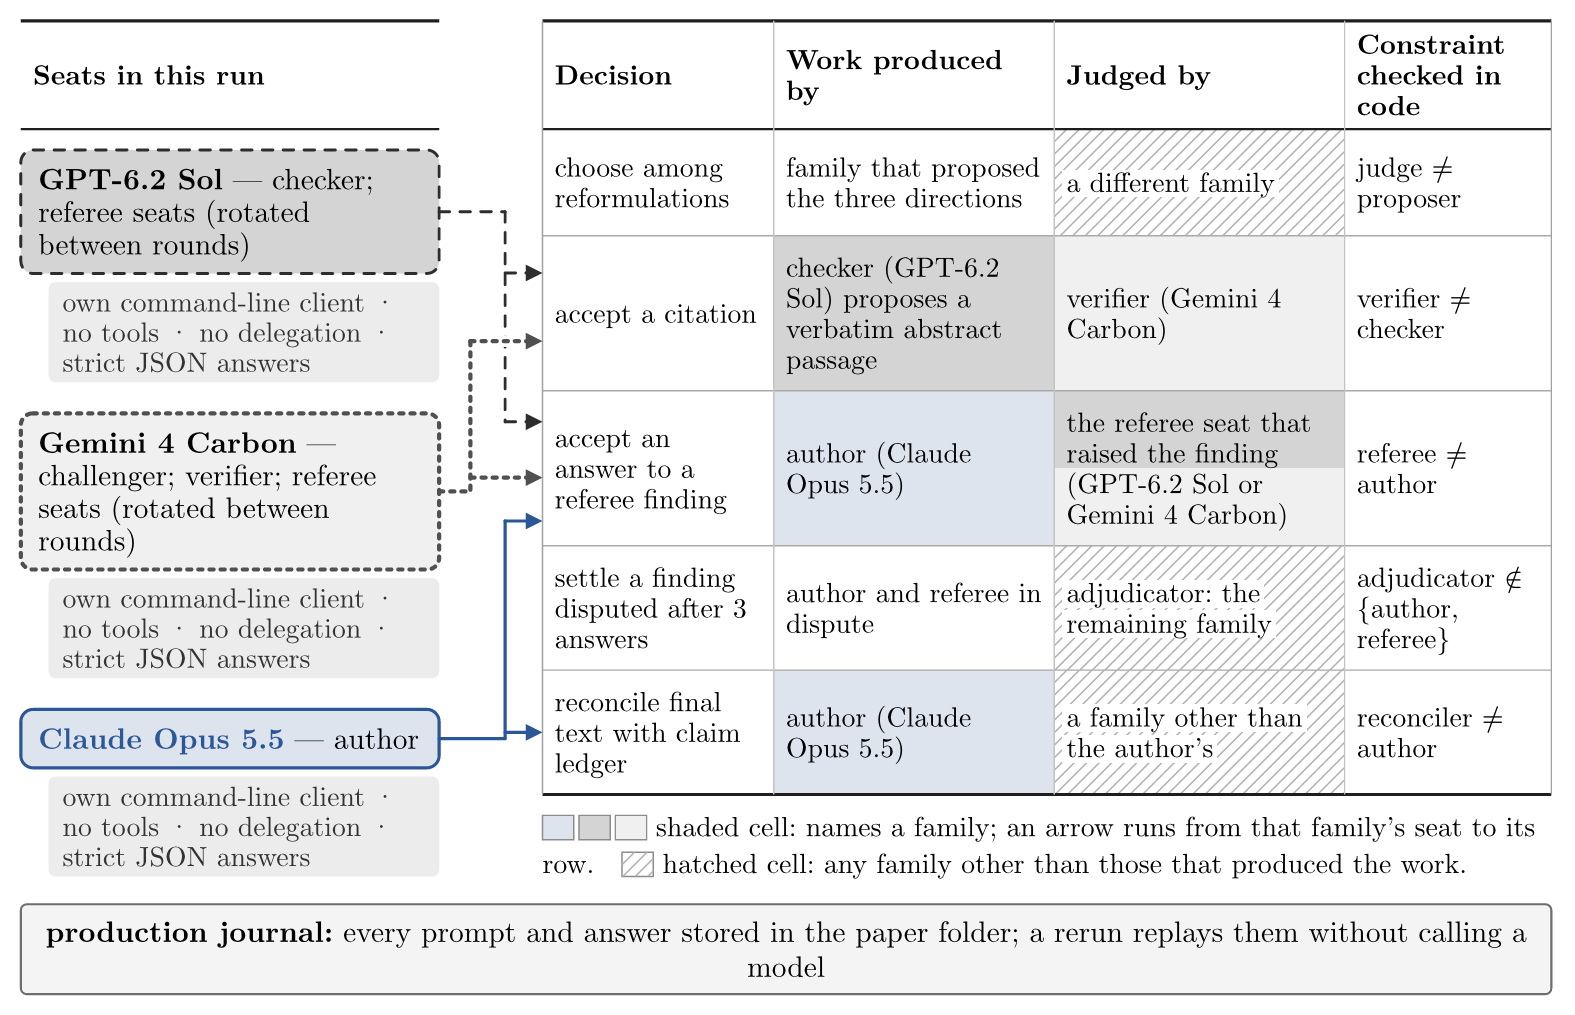
\includegraphics[width=0.95\linewidth,height=\textheight,keepaspectratio,alt={Seats
and the five decisions governed by cross-family separation of duties.
Each decision is judged by a family other than the one that produced the
work, and the rule is enforced in code, not in
prompts.}]{figures/fig1.png}
\caption{Seats and the five decisions governed by cross-family
separation of duties. Each decision is judged by a family other than the
one that produced the work, and the rule is enforced in code, not in
prompts.}\label{fig-fig1}
\end{figure}

\section{Architecture: Atomic Behaviors and the
Ladder}\label{architecture-atomic-behaviors-and-the-ladder}

Galley breaks the production of a manuscript, from seed to submission,
into a ladder of 27 atomic behaviors. The seed is the only input a
person must supply. Every later step, from reading the seed to marking
the paper ready, is the work of one of these behaviors.

\subsection{Atomic behaviors}\label{atomic-behaviors}

An atomic behavior is a unit of work that reads the paper's state, does
one thing and writes its result. It does not know which behavior runs
next.

We carried this design over from our earlier system,
\texttt{autonomio/poise}, which we built for semi-autonomous software
engineering. Galley applies the same design to a scholarly manuscript.
Each unit of work stays small, and the order of work belongs to the
scheduler, not to any behavior.

\subsection{The ladder and the
scheduler}\label{the-ladder-and-the-scheduler}

The ladder is the ordered list of the 27 atomic behaviors, in scan
order: (1) \texttt{extract}, (2) \texttt{position}, (3)
\texttt{review-idea}, (4) \texttt{reformulate}, (5)
\texttt{select-direction}, (6) \texttt{literature-review}, (7)
\texttt{analyze}, (8) \texttt{simulate}, (9) \texttt{plan}, (10)
\texttt{outline}, (11) \texttt{find-evidence}, (12) \texttt{verify},
(13) \texttt{reassess}, (14) \texttt{calibrate}, (15) \texttt{draft},
(16) \texttt{figure}, (17) \texttt{fidelity}, (18) \texttt{frame}, (19)
\texttt{referee}, (20) \texttt{close-round}, (21) \texttt{respond}, (22)
\texttt{verify-disposition}, (23) \texttt{adjudicate}, (24)
\texttt{reconcile}, (25) \texttt{reprofile}, (26) \texttt{typeset} and
(27) \texttt{ready}. The scheduler scans the ladder from the top, runs
whatever is ready, and scans again from the top whenever any behavior
settles. Readiness, which the scheduler checks against the paper's state
on each scan, decides whether a behavior runs, and position on the
ladder decides which ready behavior a scan reaches first. After a
behavior settles, the next scan can run a ready behavior higher on the
ladder. When \texttt{respond} (21) answers a finding with a new claim
that needs evidence, \texttt{find-evidence} (11) and \texttt{verify}
(12) take that claim up before the author answers again, and no behavior
needs to know that it must loop.

\subsection{Skeleton behaviors and
improvers}\label{skeleton-behaviors-and-improvers}

Minor issues do not block work. Only the seven skeleton behaviors are
required for a paper to exist: \texttt{extract} (1), \texttt{plan} (9),
\texttt{outline} (10), \texttt{draft} (15), \texttt{frame} (18),
\texttt{typeset} (26) and \texttt{ready} (27). The other twenty
behaviors are improvers. An improver can make the paper better but
cannot stop it, so small defects do not halt production.

\subsection{Isolated steps and the production
journal}\label{isolated-steps-and-the-production-journal}

Each model family runs through its own command-line client with no tools
and no delegation, and it answers in a strict JSON schema. Inside the
step, the model does not search, run code or hand work to another agent.

Galley stores every prompt and answer in the paper's folder. We call
this stored record the production journal. A rerun takes each model's
answer from the journal instead of calling the model. The journal lets a
reader inspect the run's recorded prompts and answers and replay its
model exchanges step by step.

\subsection{Building the ladder one behavior at a
time}\label{building-the-ladder-one-behavior-at-a-time}

We built the behaviors one at a time and showed each one working before
we built the next. We continued until the chain of 27 behaviors covered
the whole path from seed to submission.

\begin{figure}
\centering
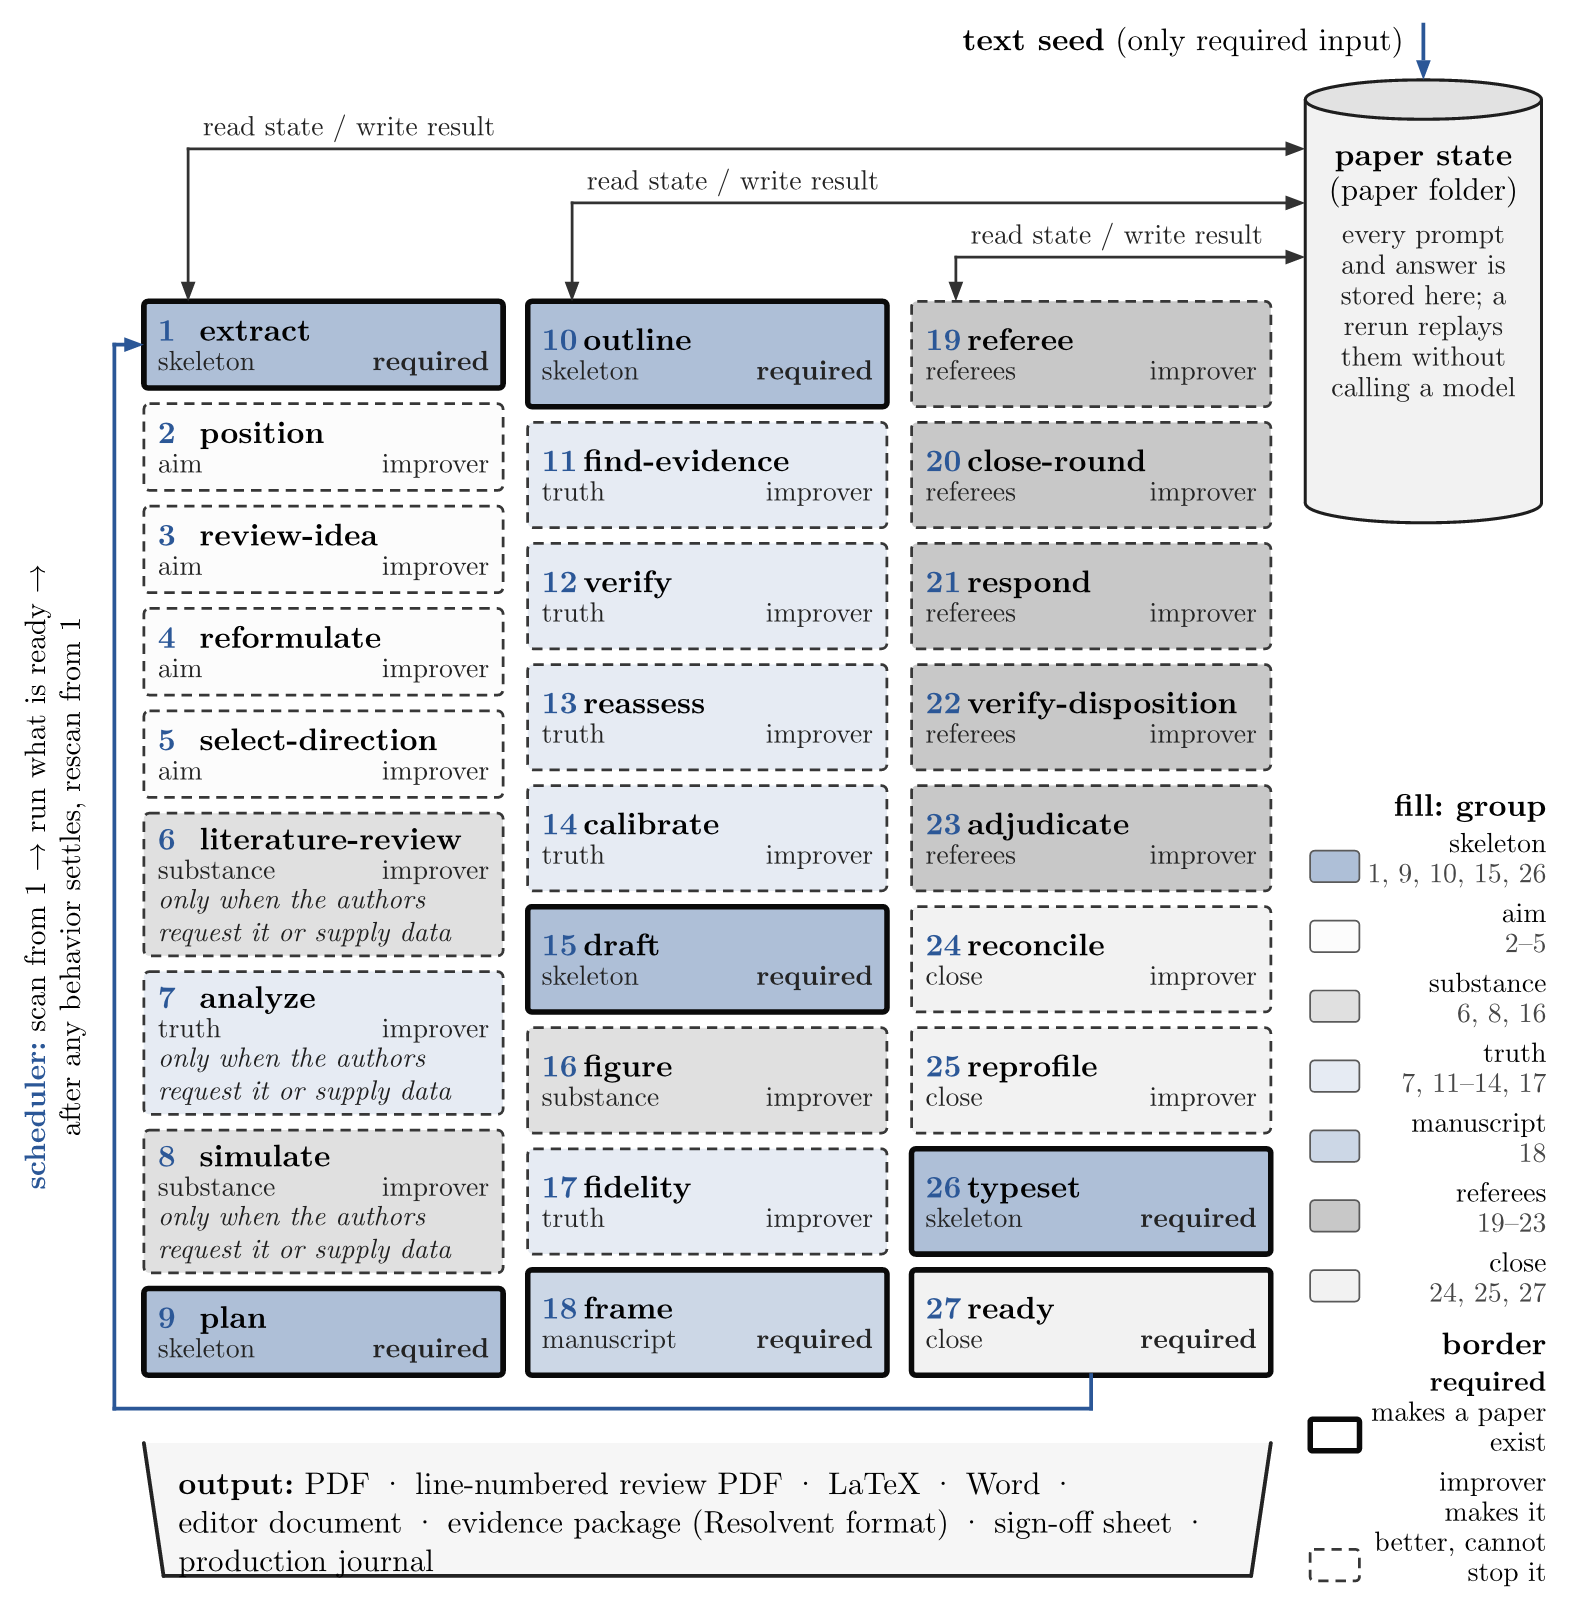
\includegraphics[width=0.95\linewidth,height=\textheight,keepaspectratio,alt={The
ladder of 27 atomic behaviors in scan order. Solid boxes are the seven
skeleton behaviors that make a paper exist; dashed boxes are improvers
that make it better but cannot stop it. The scheduler scans from
behavior 1, runs whatever is ready and rescans from 1 after any behavior
settles.}]{figures/fig2.png}
\caption{The ladder of 27 atomic behaviors in scan order. Solid boxes
are the seven skeleton behaviors that make a paper exist; dashed boxes
are improvers that make it better but cannot stop it. The scheduler
scans from behavior 1, runs whatever is ready and rescans from 1 after
any behavior settles.}\label{fig-fig2}
\end{figure}

\section{From Seed to Verified
Evidence}\label{from-seed-to-verified-evidence}

\subsection{Impact interrogation and
reformulation}\label{impact-interrogation-and-reformulation}

Before it writes any text, Galley screens the seed against a
seven-factor impact standard, the authors' own design heuristic for how
the paper should be written. Galley scores the seed on each factor,
names the weakest factor and returns one of three verdicts: worth
writing, reformulate, or no contribution. Like every improver, this
screen can redirect the paper but cannot stop it. The same seven factors
score the finished paper again.

A reformulate verdict leads to exactly three directions. Galley proposes
them. Each direction differs structurally from the other two, and each
keeps the seed's explicit commitments. Galley then chooses either the
original idea or one of the three directions. A family other than the
proposing family makes this choice.

\subsection{Filling the gaps the argument
needs}\label{filling-the-gaps-the-argument-needs}

Once Galley selects a direction, it addresses gaps in the argument.
Evidence search is the main route. Two further routes are optional, and
both run on the authors' machine.

Galley can analyze the authors' data on their machine. Galley can also
run a simulation on the authors' machine.

\subsection{Evidence search through
Canary}\label{evidence-search-through-canary}

Galley finds external evidence through Canary, the component it uses to
search OpenAlex, a fully open index of scholarly works, authors, venues
and institutions (\citeproc{ref-priem2022openalex}{Priem et al. 2022};
\citeproc{ref-priem2024openalex}{Jason et al. 2024}). Galley's source,
including its calls to Canary, is released under the MIT licence at
https://github.com/autonomio/galley. For each claim that needs external
evidence, Galley writes search queries, runs them through Canary and
considers up to a set number of candidate works. The run used a cap of
10 candidate works per claim.

At the authors' request, Canary also reviews the literature in the
background, in what we call a model-run review. The author writes a
review question. A research model plans the search of OpenAlex, screens
the candidates, reads their full texts and quotes the passage behind
each finding, and an independent model audits every finding. Each upheld
finding joins the claim ledger and the evidence package with its quoted
passage as a verified citation. A reader audits a model-run review
finding by finding, against each finding's quoted passage and its
independent audit.

\subsection{Verbatim-gated citation
verification}\label{verbatim-gated-citation-verification}

For citations from claim-level evidence search, Galley checks candidate
works against abstracts only and accepts a citation only when code
confirms that the supporting passage is copied verbatim from the cited
work's abstract. Citations from a model-run review rest instead on
full-text passages that an independent model has audited.

Two families also act on each citation from claim-level evidence search.
The checker proposes a passage for a claim. The verifier belongs to a
different family and judges the passage against that claim. Such a
citation thus needs both a verbatim match confirmed by code and a
judgment of support from the verifier. The verifier classifies each
passage as supported, narrower or not supported. A supported passage
keeps the claim and the citation as they stand. A narrower passage keeps
the citation and narrows the claim to what the passage states. Galley
rejects a citation judged not supported.

Galley takes the bibliographic record for a cited work with a DOI from
the DOI registry.

\subsection{Claims without evidence}\label{claims-without-evidence}

Galley writes claims without evidence as hypotheses. Two behaviors check
the thesis and the prose against the available evidence.

A load-bearing claim is one the thesis depends on. When such a claim
ends without evidence, the \texttt{reassess} behavior decides whether
the thesis stands, narrows or fails. The \texttt{fidelity} behavior
rewrites drafted sentences that say more than their evidence supports.

\section{Cross-Family Peer Review and
Reconciliation}\label{cross-family-peer-review-and-reconciliation}

In Galley, referees from different model families review the manuscript.
Reconciliation follows peer review. Cross-family separation of duties
decides who judges at each step. The author writes the text and answers
material findings. Another model family judges both the text and the
answers.

\subsection{Referee seats and
findings}\label{referee-seats-and-findings}

Four referee seats review the manuscript: methods, the host field,
citations and the desk editor. Each seat comes from a model family other
than the author's. The families rotate between rounds, so a seat held by
one family in a round passes to another family in the next.

Each seat can raise findings. A finding names an issue in the manuscript
and carries a severity.

\subsection{Answers and their
judgment}\label{answers-and-their-judgment}

The author answers each material finding with one of four dispositions.
A fix lists the exact edits made to the text. A rebuttal argues that the
finding does not hold. A limitation accepts the finding and states it as
a limitation of the work. The author can also request new evidence on
the finding.

The referee who raised a finding judges the answer to it. The family
that wrote an answer never decides whether that answer settles the
finding.

The evaluated run allowed up to three author answers per finding. A
finding still disputed at that cap goes to adjudication by a family
distinct from both the author's and the raising referee's.

The evaluated run allowed at most two referee rounds. The production
journal stores every finding, answer, judgment and adjudication from the
run.

\subsection{Closing reconciliation}\label{closing-reconciliation}

Review can change the text and leave the claim ledger out of step with
it. A fix can soften a sentence. A limitation can qualify a claim. An
edit in one section can remove a statement that the ledger still lists.
When this happens, the ledger records claims at a strength the text no
longer gives them.

Closing reconciliation checks the claim ledger against the post-review
text. Once peer review finishes, a family other than the author's reads
the final text against every claim in the claim ledger and assigns each
claim one of three outcomes. It confirms a claim that the text still
states as recorded. It narrows a claim to the text's wording when the
text now says less than the ledger. It drops a claim that the text no
longer states. The production journal stores each outcome with the claim
it applies to. Because reconciliation follows peer review and
adjudication, referees read the pre-reconciliation ledger, and the
typeset step renders the reconciled ledger, evidence package and
sign-off sheet only after review ends.

Reconciliation aligns recorded claims with the text through a
cross-family model judgment, and the typeset step propagates the
resulting ledger across the companion artifacts. Reconciliation works
from the recorded claims and updates the ledger rather than the text, so
an assertion that never entered the ledger lies outside its check. The
reconciling family's judgment decides which recorded claims remain in
the ledger and how the ledger states them. Claims that reconciliation
drops do not appear in the appended ledger, the evidence package or the
sign-off sheet. When the text or ledger changes, the typeset step
renders the manuscript with its appended ledger, the evidence package
and the sign-off sheet from the same revision. Those three outputs
therefore carry the same claim entries by derivation from one revision
rather than by a comparison after rendering. The ready step marks the
paper ready for submission only once every gate holds on one revision.
Code enforces the cross-family seat assignment for reconciliation, while
claim-to-text agreement on recorded claims rests on that family's
judgment rather than a code check.

\section{In-Run Calibration}\label{in-run-calibration}

In-run calibration is Galley's diagnostic audit of judgment reliability
on a manuscript's own inputs. Unlike calibration in machine learning, no
check adjusts model probabilities or decision thresholds. All three
checks belong to improver behaviors rather than the seven skeleton
behaviors (Section 4), and each runs when the paper's state makes its
behavior ready on the ladder. First, during claim-level citation
verification, code requires every proposed supporting passage to match
the cited work's OpenAlex abstract verbatim (Section 5). Second, once a
run has verified citations, the \texttt{calibrate} behavior tests the
verifier on planted defects and verified controls. Third, after peer
review finishes, a model family other than the author's reconciles the
final text against every claim in the ledger through the
\texttt{reconcile} behavior (Section 6). Verbatim matching rejects any
proposed passage that does not match the abstract, and
\texttt{reconcile} confirms, narrows or drops each ledger claim, whereas
\texttt{calibrate} only measures: it reports two rates and, as an
improver, cannot stop the paper from reaching \texttt{ready}. The
production record reports which of these behaviors ran in the evaluated
run, and Section 9 reports its citation-verification and calibration
counts. As a design choice rather than a claim of equivalent test
coverage, Galley relies on these in-run checks and keeps pre-deployment
offline test suites minimal.

The \texttt{calibrate} behavior places deliberately defective citations
(planted defects) alongside unaltered verified citations (controls), and
the verifier judges the mixed set. A planted defect is defective by
construction. Controls are drawn from this manuscript's verified
citations. A control is a citation the verifier has already accepted
during verification, so accepting it again shows consistency with that
earlier judgment, not independently established accuracy. From these
judgments \texttt{calibrate} measures two rates for this run's planted
set alone, both reported in the production record: the proportion of
planted defects the verifier catches and the proportion of unaltered
controls it wrongly rejects. The \texttt{calibrate} implementation in
Galley's source (https://github.com/autonomio/galley) defines how it
selects controls, constructs planted defects and counts each of the
verifier's three judgments, including narrower judgments, toward these
rates. Pairing defects with controls prevents a trivial verifier that
rejects every citation from appearing reliable, since such a verifier
catches every planted defect while wrongly rejecting every control. The
planted set is drawn from one manuscript's citations, and planted
defects need not resemble the errors in naturally occurring candidates,
so the rates do not estimate the verifier's accuracy beyond that set.

\begin{figure}
\centering
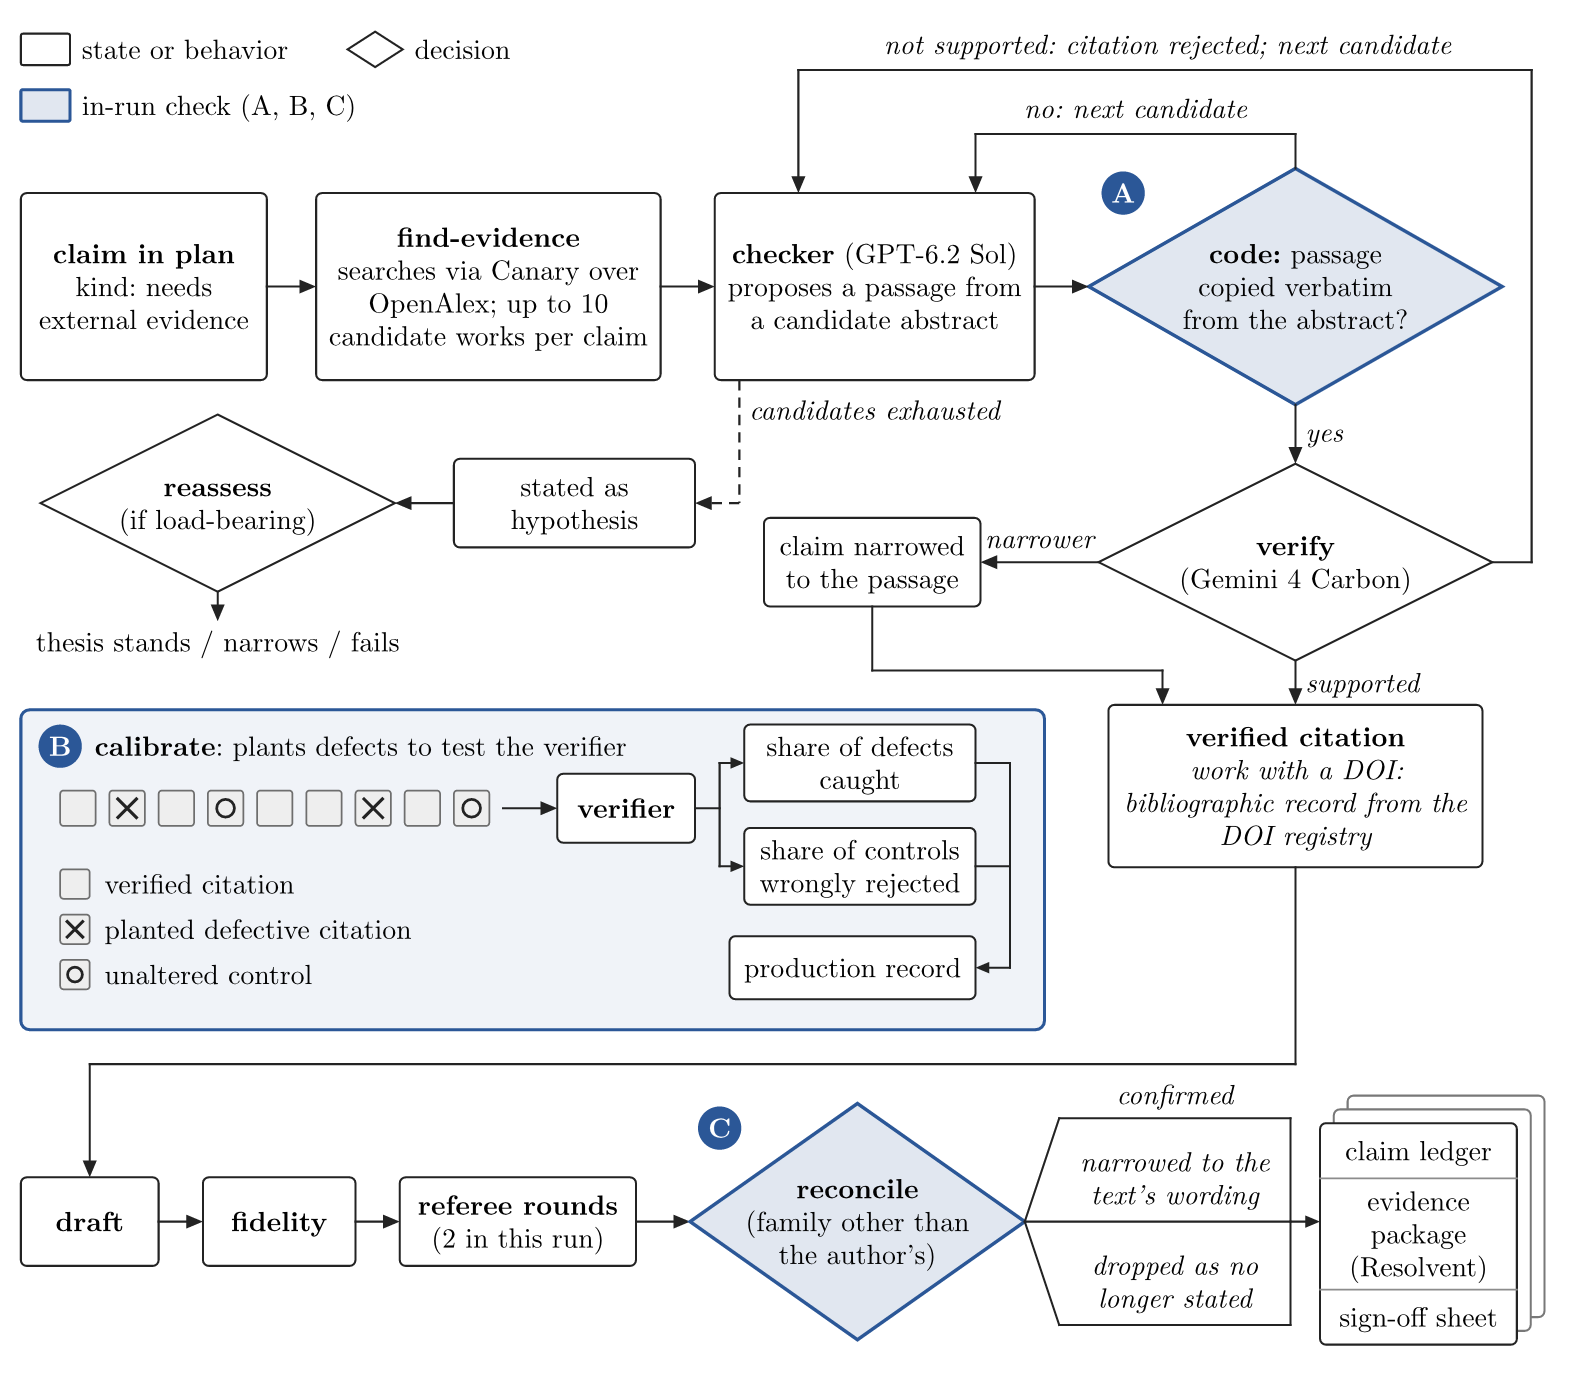
\includegraphics[width=0.95\linewidth,height=\textheight,keepaspectratio,alt={Lifecycle
of a claim that needs external evidence, with the three in-run checks
marked A (verbatim match, enforced by code), B (planted-defect
calibration) and C (cross-family reconciliation). No rates are drawn;
the production record reports them for the run.}]{figures/fig3.png}
\caption{Lifecycle of a claim that needs external evidence, with the
three in-run checks marked A (verbatim match, enforced by code), B
(planted-defect calibration) and C (cross-family reconciliation). No
rates are drawn; the production record reports them for the
run.}\label{fig-fig3}
\end{figure}

\section{Optional Human Control and
Provenance}\label{optional-human-control-and-provenance}

\subsection{Joining a run}\label{joining-a-run}

Galley lets a person join a run at any point and never requires one to.

A person can edit the manuscript directly in the editor. Galley treats
those edits as the person's revision and takes them up on the next run.

A comment in the editor becomes a thread. By default, the agents take
over the thread. A person who marks the thread \texttt{@humans} keeps it
for themselves. A person who marks it \texttt{@both} shares it with the
agents.

In an \texttt{@both} thread, the agents' edits arrive as proposed
changes. Each proposed change is marked at its place in the document,
and the person accepts or declines it.

Citation choices give a person control over which sources the paper
cites. With citation choices turned on, each claim waits for the
person's decision. The person can select candidate source a, b or c, let
Galley choose, or state the claim without a source. This run used
automatic citation.

The dial sets which steps wait for a person. Its \texttt{autonomous}
setting lets every step proceed without waiting for a person, while
leaving human edits and comment threads optional. Another setting makes
load-bearing citations and critical answers wait for the person. A
further setting makes every answer wait for the person.

\subsection{Provenance each run
leaves}\label{provenance-each-run-leaves}

Every manuscript Galley produces includes a claim ledger at the end. For
each claim the run records, the ledger gives its kind, its standing, its
origin (the seed or the system) and its sources.

Each manuscript also carries a production record generated from the
run's production journal.

The run writes a sign-off sheet alongside the manuscript. The sheet
lists what only the authors can decide: the declarations, the claims the
system added, the claims stated as hypotheses, the decisions a third
family made, and the steps that were skipped.

Each run also writes its own evidence package through the typeset
behavior, implemented in Galley's open-source repository
(https://github.com/autonomio/galley). The package holds the paper's
claims, evidence and sources in the Resolvent format. Digital-library
research may already model provenance at the level of individual claims,
holding each assertion, its evidence and its source as one
machine-readable record; how the Resolvent format relates to such models
remains an open question. The evidence for a cited claim is the passage
that code confirmed is copied verbatim from the cited work's abstract
and that the verifier judged. A cited work with a DOI takes its
bibliographic record from the DOI registry. After peer review, a family
other than the author's reconciles the recorded claims in the ledger
against the final text, and the typeset behavior writes the package from
that reconciled state (Section 6).

The claim ledger and the production record appear in the manuscript
itself. The sign-off sheet, the evidence package and the production
journal are written to the paper's folder. Galley does not publish them,
so readers can inspect a run's files only where its authors release that
folder. The journal stores every prompt and answer of the run. For each
candidate citation it holds the verifier's prompt, with the claim and
the passage exactly as the verifier received them, and the verifier's
judgment. A rerun replays the journal without calling a model.

\section{Evaluation: A Self-Referential
Run}\label{evaluation-a-self-referential-run}

We evaluate Galley through one self-referential run. Galley produced
this manuscript, which introduces Galley, from the authors' seed. The
seed asked what sets very high-impact papers apart and presented Galley
as a semi-autonomous, multi-agent editor built from atomic behaviors,
each proven before the next is built. The run proposed three directions
and selected one that recentres the paper on cross-family separation of
duties and in-run calibration; the selecting family was not the family
that proposed the directions. Galley ran with the dial set to
autonomous, so no step waited for a person. Every count and rate in this
section comes from the production record, which Galley generates from
the run's production journal. The journal stores every prompt and answer
of the run in the paper's folder, and a rerun with Galley's source
(https://github.com/autonomio/galley, MIT licence) replays them without
calling a model, so each governed decision, such as the selection of a
direction or the adjudication of a finding, is recorded as the stored
answer of the seat that made it. Typesetting renders the claim ledger at
the end of this manuscript from the surviving recorded claims, listing
whether the seed or the system added each claim alongside its sources
and reconciled standing. The run also writes an evidence package of
claims, evidence and sources in the Resolvent format.

The run used automatic citation. The settings allowed 2 referee rounds,
capped answers at 3, and allowed up to 10 candidate works per claim.

The run took 3.5 wall-clock hours from seed to this manuscript and made
148 model calls. The run made 73 calls to Claude, 37 to GPT and 38 to
Gemini. The run read 3.3 million input tokens and wrote 2003 thousand
output tokens. Galley ran 24 behaviors.

The final argument contains 44 claims. Of these, 18 came from the seed
and the system added 26. Galley narrowed 9 claims. Of the claims marked
as needing external evidence, 4 ended without verified evidence and are
stated as hypotheses; claims marked as the authors' own work or as
premises do not seek external citations.

The evidence search screened 278 candidate works. Galley verified 23
citations. It rejected 13 proposed citations. During calibration, Galley
detected 6 of 6 planted defects and accepted 2 of 2 controls.

Over 2 referee rounds, the referee seats raised 87 findings, and 76 of
them were material or critical. Galley resolved 76 of the material or
critical findings. Galley adjudicated 16 findings.

In this paper, submission-ready means that Galley's own gates held on
one revision of the manuscript. It does not mean that outside reviewers
accepted the paper, and it does not replace the authors' review of the
sign-off sheet. The evaluation reports governed decisions as counts; no
single decision has been audited independently of the run's production
journal. That sheet lists what only the authors can decide:
declarations, the 26 claims the system added, claims stated as
hypotheses, decisions a third family made and skipped steps.

\section{Limitations}\label{limitations}

This work leaves three questions about impact open. We do not test
whether papers that Galley produces go on to high citation impact. We
also do not test whether Galley can produce such papers at high volume,
or whether the seven-factor profile predicts impact. We state all three
as open hypotheses.

Methodological and evaluation scope are similarly bounded. The evidence
here comes from one run on one seed, with one assignment of model
families to seats and no baseline system; we do not test whether
cross-family separation of duties catches more errors than single-family
review, we do not evaluate the human-in-the-loop controls with users,
and we do not check the generated package against any venue's submission
requirements. We also do not compare the in-run checks against a
pre-deployment offline test suite, so this work does not establish
whether they catch the failures that an offline suite would detect.
Separate model families may share failure modes, so one family's review
need not catch another's errors. No person independently audited
citation support, manuscript quality or the settlement of referee
findings by fix, rebuttal, limitation or third-family adjudication. No
person verified that the reconciled claim ledger, evidence package and
sign-off sheet match the final text. Because the seed describes Galley
itself, the seed's claims about how Galley works are the authors' own
and rest on no external source, and the single run gives no independent
test of the model-run review, data analysis or simulation behaviors.
Only a model-run review reads full texts, with an independent model
auditing each finding; outside one, Galley checks each citation against
the cited work's abstract as found in OpenAlex. A work with no abstract
there cannot supply a verified citation. A claim that rests on
implementation choices, methods or results reported only in full text is
either narrowed to what an abstract states or left as a hypothesis.

\section{What This Opens}\label{what-this-opens}

Six studies could build on cross-family separation of duties and in-run
calibration. Study materials could include a production journal, a claim
ledger and an evidence package.

The first is a controlled comparison of cross-family and single-family
verification and review. For each judging behavior, such as citation
verification or the judging of referee answers, the study would replay
identical upstream steps from the journal and cross the producing family
with the judging family across all nine pairings of three families, so
no other seat enters the comparison. The study would report all nine
cell means and estimate the average departure of the three same-family
cells from what additive producer and judge effects predict;
pairing-specific effects can also contribute to that contrast.
Separating family matching from reuse of the identical model would
require identical-model and distinct-model pairings within each family.
Alongside in-run planted-defect, control and referee metrics, blinded
human annotators would audit surviving claim--citation accuracy and
manuscript quality.

The second would extend in-run calibration to full texts, analyses,
simulations and figures. The study could pair planted defects with
unaltered controls in full-text passages, numerical analysis outputs,
simulation inputs and results, and compiled figures. The study would
compare the verifier's performance on these materials with its
performance on citation checks.

The third is a user study of the human controls. It would observe people
using the dial, \texttt{@both} threads with their proposed changes, and
the sign-off sheet. It would measure which decisions people take over
and which proposed changes they accept. It would also measure whether
the sign-off sheet directs their attention to the claims the system
added and the claims stated as hypotheses.

The fourth is a prospective science-of-science test of the seven-factor
profile. The study would score seeds and finished papers before
publication and track citations to the papers afterward. The study would
test whether the profile predicts subsequent citations.

The fifth is a seed-to-preprint benchmark. Participating systems would
run the same seeds, and blinded assessors would use each output's claim
ledger and evidence package to locate claims and source passages, judge
support against a shared rubric, and report coverage of the seed's
substantive claims alongside claims narrowed, dropped or left as
hypotheses.

The sixth applies the pattern outside scholarly writing. We hypothesize
that cross-family separation of duties transfers to clinical guidelines,
legal briefs and intelligence assessments. The study could use at least
three model families, assign claim writing and verification to different
families, and record prompts and answers in a journal.

\section*{Appendix A: Claim ledger}\label{appendix-a-claim-ledger}
\addcontentsline{toc}{section}{Appendix A: Claim ledger}

Every claim of the final argument, as the claim ledger holds it: its
kind, its standing, where it came from, and the verified sources it
rests on. Identifiers are the ledger's own and need not be consecutive.

\begin{itemize}
\tightlist
\item
  \textbf{C1} (background; narrowed to its evidence; from the seed)
  (\citeproc{ref-sarigol2014predicting}{Sarigöl et al. 2014};
  \citeproc{ref-yan2009applying}{Yan and Ding 2009}). Citation outcomes
  have been linked to the authors' position in coauthorship networks, a
  factor outside a paper's content.
\item
  \textbf{C4} (contribution, load-bearing; the authors' own work; from
  the seed). From a text seed, Galley, a semi-autonomous, multi-agent
  scholarly editor, produces a package that is submission-ready under
  its own gates on one revision. The package includes the manuscript as
  a PDF, a line-numbered review PDF, LaTeX and Word, together with its
  claim ledger, evidence package, sign-off sheet and production journal.
\item
  \textbf{C6} (method; the authors' own work; from the seed). Before
  writing the manuscript, Galley screens the seed against the authors'
  seven-factor impact heuristic, names the weakest factor and gives a
  verdict. On a reformulate verdict, it proposes three structurally
  different directions that keep the seed's explicit commitments. A
  family other than the proposer chooses the original idea or one of the
  three directions. Galley then addresses gaps through evidence search
  and can optionally analyze the authors' data or run a simulation on
  their machine.
\item
  \textbf{C7} (method; the authors' own work; from the seed). Galley
  searches OpenAlex through Canary, writing queries for each claim that
  needs external evidence and considering up to a fixed number of
  candidate works, ten in this run. At the authors' request, Canary runs
  a model-run literature review. Each finding upheld by an independent
  model audit joins the claim ledger with its quoted passage.
\item
  \textbf{C9} (contribution; premise; from the seed). This paper does
  not test whether papers produced by galley go on to high citation
  impact, whether galley can produce such papers at high volume, or
  whether the seven-factor profile predicts impact. All three are stated
  as open hypotheses.
\item
  \textbf{C10} (method; the authors' own work; from the seed). Each run
  writes its own evidence package, holding the paper's claims, evidence
  and sources in the Resolvent format.
\item
  \textbf{C11} (method, load-bearing; the authors' own work; from the
  seed). Peer review is run by agents from different families. Referee
  seats for methods, the host field, citations and the desk editor are
  drawn from families other than the author's and rotated between
  rounds, and each finding they raise carries a severity. The author
  answers each material finding by fixing it with exact edits, rebutting
  it, stating it as a limitation, or asking for new evidence. The
  referee who raised the finding judges the answer. If a finding is
  still disputed after a cap of answers (three in this run), a third
  family adjudicates. This run used two referee rounds, and every
  exchange is kept in the journal.
\item
  \textbf{C12} (method; the authors' own work; from the seed). When a
  person shares a thread with the agents (@both), the agents' edits
  arrive as proposed changes marked at their place in the document, and
  the person accepts or declines each one. This paper describes the
  mechanism but does not test it with users.
\item
  \textbf{C14} (method; the authors' own work; from the seed). With
  citation choices turned on, each claim waits for the person to pick
  one of its candidate sources (a, b, c), let the system pick, or state
  the claim without a source. This run used automatic citation.
\item
  \textbf{C15} (method; the authors' own work; from the seed). A person
  can join at any point but is never required to. Edits made in the
  editor become their revision on the next run. A comment becomes a
  thread that the agents take over by default, that the person keeps
  (@humans), or that both share (@both). A dial can make load-bearing
  citations and critical answers, or every answer, wait for the person.
\item
  \textbf{C17} (method, load-bearing; the authors' own work; from the
  seed). Galley runs several model families in separate seats. In this
  run Claude Opus 5.5 is the author, GPT-6.2 Sol is the checker, and
  Gemini 4 Carbon is the challenger and the verifier. Referees come from
  the families other than the author's, and the adjudicator comes from
  the family that is neither the author's nor the referee's.
\item
  \textbf{C18} (method; the authors' own work; from the seed). Galley is
  organized around atomic behaviors, each of which reads the paper's
  state, does one thing and writes its result. The authors carried this
  design over from their earlier system autonomio/poise, which they
  built for semi-autonomous software engineering.
\item
  \textbf{C19} (method, load-bearing; the authors' own work; from the
  seed). Galley breaks seed-to-submission production into a ladder of 27
  atomic behaviors. A scheduler scans the ladder from the top, runs
  whatever is ready, and scans again from the top whenever anything
  settles; no behavior knows what comes next. The text seed is the only
  input a person must supply.
\item
  \textbf{C20} (method; the authors' own work; from the seed). Work is
  not blocked by minor issues. Only the seven skeleton behaviors
  (extract, plan, outline, draft, frame, typeset, ready) are required
  for a paper to exist. Every other behavior is an improver that can
  make the paper better but cannot stop it, so small defects do not halt
  production.
\item
  \textbf{C22} (method, load-bearing; the authors' own work; from the
  seed). Galley checks its reliability inside each run, on that
  manuscript's actual inputs. Code enforces verbatim matching of
  passages against abstracts, the calibrate behavior plants defects to
  test the verifier, and a different family reconciles the final text.
  These in-run checks take the place of long offline test suites run
  before deployment, so galley keeps its offline tests minimal.
\item
  \textbf{C24} (method; the authors' own work; from the seed). The
  authors built the behaviors one at a time and showed each one working
  before building the next, until the 27-behavior chain covered the
  whole path from seed to submission.
\item
  \textbf{C25} (contribution; the authors' own work; from the seed).
  Galley is released as @autonomio/galley 0.1.0 under the MIT licence,
  with source code at https://github.com/autonomio/galley.
\item
  \textbf{C26} (method, load-bearing; the authors' own work; from the
  seed). The evaluation is a single self-referential run. Galley
  produced this manuscript, which introduces galley, from the authors'
  seed with the dial set to autonomous, so no step waited for a person.
  The production record generated from the run's journal reports what
  each behavior did. `Submission-ready' means galley's own gates held on
  one revision, not that outside reviewers accepted the paper.
\item
  \textbf{C27} (background; narrowed to its evidence; added by the
  system) (\citeproc{ref-yang2026deepsurvey}{Yang et al. 2026}). Agent
  systems already automate parts of scholarly production: writing
  scientific surveys (DeepSurvey) and checking that citations support
  the claims they are attached to.
\item
  \textbf{C28} (background; hypothesis: no verified evidence; added by
  the system). Interactive provenance visualization can show authors
  which parts of a text an LLM contributed (HaLLMark).
\item
  \textbf{C29} (background; hypothesis: no verified evidence; added by
  the system). Prior multi-agent scholarly systems assign drafting,
  reviewing and verifying roles through prompts, and do not state a rule
  that the model doing the evaluation must come from a different model
  family than the model that produced the work.
\item
  \textbf{C30} (background, load-bearing; supported; added by the
  system) (\citeproc{ref-panickssery2024llm}{Panickssery et al. 2024};
  \citeproc{ref-chen2025beyond}{Chen et al. 2025}). LLMs used as
  evaluators tend to rate their own outputs more favorably than outputs
  from other models (self-preference bias).
\item
  \textbf{C31} (background; narrowed to its evidence; added by the
  system) (\citeproc{ref-kugblenu2007separation}{Kugblenu and Asim
  2007}). Separation of duties is an established security principle in
  organizations.
\item
  \textbf{C32} (background, load-bearing; narrowed to its evidence;
  added by the system) (\citeproc{ref-lai2026hallucinatio}{Lai et al.
  2026}; \citeproc{ref-linardon2026fluency}{Linardon et al. 2026}).
  LLM-generated scholarly text can contain misattributed citations.
\item
  \textbf{C33} (background; narrowed to its evidence; added by the
  system) (\citeproc{ref-andrews2006using}{Andrews et al. 2006};
  \citeproc{ref-ma2018deepmutation}{Ma et al. 2018}). In mutation
  analysis in software testing, planting known defects and counting how
  many are caught is an established way to estimate sensitivity.
\item
  \textbf{C34} (method, load-bearing; the authors' own work; added by
  the system). For citations from claim-level evidence search, Galley
  requires a code-confirmed verbatim match to the cited work's abstract.
  The checker proposes the passage and a verifier from another family
  judges it supported, narrower or not supported. Galley narrows the
  claim for a narrower judgment and rejects the citation for a
  not-supported judgment. Model-run review citations use independently
  audited full-text passages. Galley takes the bibliographic record for
  a cited work with a DOI from the DOI registry.
\item
  \textbf{C35} (method, load-bearing; the authors' own work; added by
  the system). The calibrate behavior plants defective citations and
  unaltered controls among the verified citations and measures how many
  defects the verifier catches and how many controls it wrongly rejects.
  The production record reports both rates for this run.
\item
  \textbf{C36} (method, load-bearing; the authors' own work; added by
  the system). After peer review, a family other than the author's
  compares each recorded claim with the final text and confirms it,
  narrows it to the text's wording or drops it. The ledger, evidence
  package and sign-off sheet carry the same reconciled claim entries
  from one revision. Agreement with the manuscript rests on the
  reconciling family's judgment about the recorded claims.
\item
  \textbf{C37} (method, load-bearing; the authors' own work; added by
  the system). Each family uses its own command-line client without
  tools or delegation and answers in a strict JSON schema. Galley stores
  every prompt and answer in the paper's folder, and a rerun replays the
  recorded model exchanges step by step without calling a model. Readers
  can inspect the journal where the authors release the folder.
\item
  \textbf{C38} (method; the authors' own work; added by the system).
  Every manuscript ends with its claim ledger, giving each claim's kind,
  standing, origin (seed or system) and sources, and with a production
  record generated from the run's journal. The run also writes a
  sign-off sheet of what only the authors can decide: declarations,
  claims the system added, claims stated as hypotheses, decisions a
  third family made, and skipped steps.
\item
  \textbf{C39} (method; the authors' own work; added by the system).
  Claims without evidence are written as hypotheses. When a load-bearing
  claim ends up without evidence, the reassess behavior decides whether
  the thesis stands, narrows or fails, and the fidelity behavior
  rewrites drafted sentences that say more than their evidence.
\item
  \textbf{C40} (novelty, load-bearing; the authors' own work; added by
  the system). Galley enforces cross-family separation of duties in code
  through seat assignment. A different family selects among
  reformulations, verifies claim-level citation passages, judges referee
  responses, adjudicates disputes and reconciles the final manuscript.
\item
  \textbf{C41} (contribution, load-bearing; the authors' own work; added
  by the system). Cross-family separation of duties, combined with
  in-run calibration, is a governance pattern for multi-agent writing
  that has to stay tied to evidence, and it can be used without galley's
  other components. It needs at least three model families, so that an
  adjudicator can come from neither the author's nor the referee's
  family, plus a journal of prompts and answers.
\item
  \textbf{C42} (method; the authors' own work; added by the system). The
  paper does not test whether cross-family separation catches more
  errors than single-family review or evaluate the human controls with
  users. Galley checks citations against OpenAlex abstracts outside
  model-run reviews, which use full-text passages and an independent
  model audit. The evidence comes from one run on one seed, with one
  family assignment and no baseline system.
\item
  \textbf{C43} (background; supported; added by the system)
  (\citeproc{ref-chen2025beyond}{Chen et al. 2025}). Large language
  models used as evaluators tend to rate their own outputs more
  favorably than outputs from other models.
\item
  \textbf{C44} (background; supported; added by the system)
  (\citeproc{ref-priem2022openalex}{Priem et al. 2022};
  \citeproc{ref-priem2024openalex}{Jason et al. 2024}). OpenAlex is a
  fully open index of scholarly works, authors, venues and institutions.
\item
  \textbf{C45} (background; narrowed to its evidence; added by the
  system) (\citeproc{ref-hoque2024hallmark}{Hoque et al. 2024}).
  HaLLMark is a tool that visualizes provenance in human--LLM
  co-writing.
\item
  \textbf{C46} (background; hypothesis: no verified evidence; added by
  the system). Multi-agent LLM systems for scholarly work, such as
  SciSage, DeepReviewer 2.0 and DeepSciVerify, automate manuscript
  writing, peer review or scientific claim verification by dividing
  these tasks among role-specialized agents.
\item
  \textbf{C47} (background; narrowed to its evidence; added by the
  system) (\citeproc{ref-siddiqui2026draftmarks}{Siddiqui et al. 2026};
  \citeproc{ref-laban2024beyond}{Laban et al. 2024}). Prior HCI work on
  human--AI co-writing records provenance of what an LLM generated in a
  document.
\item
  \textbf{C49} (background; hypothesis: no verified evidence; added by
  the system). Prior digital-library research may already model
  scholarly provenance at the level of individual claims, representing
  each assertion, its evidence and its source in one machine-readable
  record.
\item
  \textbf{C50} (background; supported; added by the system)
  (\citeproc{ref-verga2024replacing}{Verga et al. 2024}). Panels of LLM
  evaluators composed of models from disjoint model families have been
  used to judge model outputs, and such panels show less intra-model
  bias than a single large judge model (Verga et al., 2024, Panel of LLm
  evaluators, PoLL).
\item
  \textbf{C51} (background; supported; added by the system)
  (\citeproc{ref-lu2024scientist}{Lu et al. 2024};
  \citeproc{ref-yamada2025scientistv2}{Yamada et al. 2025}). Agentic LLM
  systems already generate complete research papers end to end; for
  example, The AI Scientist (Lu et al., 2024) generates research ideas,
  writes code, runs experiments, writes a full scientific paper and
  evaluates it with a simulated review process.
\item
  \textbf{C52} (background; narrowed to its evidence; added by the
  system) (\citeproc{ref-walters2023fabrication}{Walters and Wilder
  2023}; \citeproc{ref-misra2026detecting}{Misra and Udandarao 2026}).
  Large language models produce fabricated bibliographic citations, or
  real citations with errors.
\item
  \textbf{C53} (background; narrowed to its evidence; added by the
  system) (\citeproc{ref-hariri2018exploring}{Hariri 2018};
  \citeproc{ref-andrade2019analyzing}{Andrade et al. 2019}). Mutation
  analysis assesses the adequacy of test data by introducing small
  syntactic faults (mutants) into a program.
\end{itemize}

\section*{Use of AI and production
record}\label{use-of-ai-and-production-record}
\addcontentsline{toc}{section}{Use of AI and production record}

This manuscript was produced with galley 0.1.0 (MIT licence,
https://github.com/autonomio/galley) from a seed text written by the
author. Claude Opus 5.5 extracted the seed's claims, planned the
argument, drafted every section and answered the referees. GPT-6.2 Sol
wrote the literature searches, selected candidate passages and checked
each section against its claims. Gemini 4 Carbon challenged the idea
before drafting and verified every citation against the passage it rests
on. Referee reports came from GPT-6.2 Sol and Gemini 4 Carbon, never
from the family that drafted the text, and each answer to a material
finding was verified by the referee family that raised it. Literature
search ran through Canary over OpenAlex; bibliographic records come from
the DOI registries. No model reviewed its own work. The production
journal that accompanies this manuscript records every step, model call,
verdict and decision with its time, and the evidence package holds each
claim with the verbatim passage and verdict behind every citation.

{\def\LTcaptype{none} % do not increment counter
\begin{longtable}[]{@{}
  >{\raggedright\arraybackslash}p{(\linewidth - 2\tabcolsep) * \real{0.5000}}
  >{\raggedright\arraybackslash}p{(\linewidth - 2\tabcolsep) * \real{0.5000}}@{}}
\toprule\noalign{}
\begin{minipage}[b]{\linewidth}\raggedright
Production record
\end{minipage} & \begin{minipage}[b]{\linewidth}\raggedright
\end{minipage} \\
\midrule\noalign{}
\endhead
\bottomrule\noalign{}
\endlastfoot
Model calls & 148 (Claude 73, GPT 37, Gemini 38) \\
Tokens & 3.3 M in, 2003 k out \\
Claims & 44 (18 from the seed, 26 added; 9 narrowed; 4 stated as
hypotheses) \\
Works screened & 278 \\
Citations & 23 verified, 13 rejected \\
Referee findings & 87 (76 material or critical; 76 resolved; 16
adjudicated) over 2 round(s) \\
Verifier calibration & 6 of 6 planted defective citations caught; 2 of 2
unaltered controls accepted \\
\end{longtable}
}

\section*{Data and code availability}\label{data-and-code-availability}
\addcontentsline{toc}{section}{Data and code availability}

galley's source code, including the behaviors that produced this
manuscript, is available under the MIT licence at
https://github.com/autonomio/galley. Every claim in this manuscript, the
evidence it rests on and the verbatim passages of its sources are
available as an evidence package accompanying it (claims, evidence and
sources in the Resolvent format).

\section*{Competing interests}\label{competing-interests}
\addcontentsline{toc}{section}{Competing interests}

To be declared by the author.

\section*{Funding}\label{funding}
\addcontentsline{toc}{section}{Funding}

To be declared by the author.

\section*{References}\label{references}
\addcontentsline{toc}{section}{References}

\protect\phantomsection\label{refs}
\begin{CSLReferences}{1}{1}
\bibitem[\citeproctext]{ref-andrade2019analyzing}
Andrade, Stevão A., Claudinei Brito Junior, Misael Júnior, Ana Claudia
Marciel, Gabriel Abdalla, and Márcio E. Delamaro. 2019. {``Analyzing the
Effectiveness of One-Op Mutation against the Minimal Set of Mutants.''}
\emph{Proceedings of the IV Brazilian Symposium on Systematic and
Automated Software Testing}, September 23, 22--31.
\url{https://doi.org/10.1145/3356317.3356321}.

\bibitem[\citeproctext]{ref-andrews2006using}
Andrews, J.H., L.C. Briand, Y. Labiche, and A.S. Namin. 2006. {``Using
Mutation Analysis for Assessing and Comparing Testing Coverage
Criteria.''} \emph{IEEE Transactions on Software Engineering} 32 (8):
608--24. \url{https://doi.org/10.1109/tse.2006.83}.

\bibitem[\citeproctext]{ref-chen2025beyond}
Chen, Zhi-Yuan, Hao Wang, Xinyu Zhang, Enrui Hu, and Yankai Lin. 2025.
{``Beyond the Surface: Measuring Self-Preference in LLM Judgments.''}
\emph{Proceedings of the 2025 Conference on Empirical Methods in Natural
Language Processing}, 1653--72.
\url{https://doi.org/10.18653/v1/2025.emnlp-main.86}.

\bibitem[\citeproctext]{ref-hariri2018exploring}
Hariri, Farah. 2018. {``Exploring Design Decisions for Mutation
Testing.''} \emph{Illinois Digital Environment for Access to Learning
and Scholarship (University of Illinois at Urbana-Champaign)}.
\url{https://openalex.org/W3094413649}.

\bibitem[\citeproctext]{ref-hoque2024hallmark}
Hoque, Md Naimul, Tasfia Mashiat, Bhavya Ghai, et al. 2024. {``The
HaLLMark Effect: Supporting Provenance and Transparent Use of Large
Language Models in Writing with Interactive Visualization.''}
\emph{Proceedings of the CHI Conference on Human Factors in Computing
Systems}, May 11, 1--15. \url{https://doi.org/10.1145/3613904.3641895}.

\bibitem[\citeproctext]{ref-priem2024openalex}
Jason, Priem, Piwowar Heather, Justin Barrett, et al. 2024. {``OpenAlex
Snapshot.''} Zenodo, October 16.
\url{https://doi.org/10.5281/ZENODO.13941457}.

\bibitem[\citeproctext]{ref-kugblenu2007separation}
Kugblenu, Francis M., and Memon Asim. 2007. {``Separation of Duty in
Role Based Access.''} \emph{DiVA (Digitala Vetenskapliga Arkivet)}.
\url{https://openalex.org/W1125997174}.

\bibitem[\citeproctext]{ref-laban2024beyond}
Laban, Philippe, Jesse Vig, Marti Hearst, Caiming Xiong, and Chien-Sheng
Wu. 2024. {``Beyond the Chat: Executable and Verifiable Text-Editing
with LLMs.''} \emph{Proceedings of the 37th Annual ACM Symposium on User
Interface Software and Technology}, October 11, 1--23.
\url{https://doi.org/10.1145/3654777.3676419}.

\bibitem[\citeproctext]{ref-lai2026hallucinatio}
Lai, Ke En, Nuremma Mustaffa, Christopher Nigel Preece, and Foo Yeu
Wong. 2026. {``Hallucinations in Large Language Models within Academic
Contexts: A Systematic Review.''} \emph{Journal of Science and
Technology Policy Management}, July 22, 1--28.
\url{https://doi.org/10.1108/jstpm-01-2026-0015}.

\bibitem[\citeproctext]{ref-linardon2026fluency}
Linardon, Jake, Mariel Messer, Cleo Anderson, et al. 2026. {``Fluency
Without Fidelity: Errors in Citation-Attributed Claims in Large Language
Model-Generated Literature Reviews in Mental Health.''} \emph{Journal of
Technology in Behavioral Science}, ahead of print, April 20.
\url{https://doi.org/10.1007/s41347-026-00630-6}.

\bibitem[\citeproctext]{ref-lu2024scientist}
Lu, Chris, Cong Lu, Robert Tjarko Lange, Jakob Foerster, Jeff Clune, and
David Ha. 2024. {``The AI Scientist: Towards Fully Automated Open-Ended
Scientific Discovery.''} Preprint, arXiv.
\url{https://doi.org/10.48550/ARXIV.2408.06292}.

\bibitem[\citeproctext]{ref-ma2018deepmutation}
Ma, Lei, Fuyuan Zhang, Jiyuan Sun, et al. 2018. {``DeepMutation:
Mutation Testing of Deep Learning Systems.''} \emph{2018 IEEE 29th
International Symposium on Software Reliability Engineering (ISSRE)},
October, 100--111. \url{https://doi.org/10.1109/issre.2018.00021}.

\bibitem[\citeproctext]{ref-misra2026detecting}
Misra, Nipun, and Vikranth Udandarao. 2026. {``Detecting Citation
Hallucinations in Large Language Model Outputs (Student Abstract).''}
\emph{Proceedings of the AAAI Conference on Artificial Intelligence} 40
(48): 41325--27. \url{https://doi.org/10.1609/aaai.v40i48.42257}.

\bibitem[\citeproctext]{ref-panickssery2024llm}
Panickssery, Arjun, Samuel Bowman, and Shi Feng. 2024. {``LLM Evaluators
Recognize and Favor Their Own Generations.''} \emph{Advances in Neural
Information Processing Systems 37}, 68772--802.
\url{https://doi.org/10.52202/079017-2197}.

\bibitem[\citeproctext]{ref-priem2022openalex}
Priem, Jason, Heather Piwowar, and Richard Orr. 2022. {``OpenAlex: A
Fully-Open Index of Scholarly Works, Authors, Venues, Institutions, and
Concepts.''} Preprint, arXiv.
\url{https://doi.org/10.48550/ARXIV.2205.01833}.

\bibitem[\citeproctext]{ref-sarigol2014predicting}
Sarigöl, Emre, René Pfitzner, Ingo Scholtes, Antonios Garas, and Frank
Schweitzer. 2014. {``Predicting Scientific Success Based on Coauthorship
Networks.''} \emph{EPJ Data Science} 3 (1).
\url{https://doi.org/10.1140/epjds/s13688-014-0009-x}.

\bibitem[\citeproctext]{ref-siddiqui2026draftmarks}
Siddiqui, Momin N., Nikki Nasseri, Adam J. Coscia, Roy Pea, and Hari
Subramonyam. 2026. {``DraftMarks: Enhancing Transparency in Human-AI
Co-Writing Through Interactive Skeuomorphic Process Traces.''}
\emph{Proceedings of the 2026 CHI Conference on Human Factors in
Computing Systems}, April 13, 1--22.
\url{https://doi.org/10.1145/3772318.3791109}.

\bibitem[\citeproctext]{ref-verga2024replacing}
Verga, Pat, Sebastian Hofstatter, Sophia Althammer, et al. 2024.
{``Replacing Judges with Juries: Evaluating LLM Generations with a Panel
of Diverse Models.''} Preprint, arXiv.
\url{https://doi.org/10.48550/ARXIV.2404.18796}.

\bibitem[\citeproctext]{ref-walters2023fabrication}
Walters, William H., and Esther Isabelle Wilder. 2023. {``Fabrication
and Errors in the Bibliographic Citations Generated by ChatGPT.''}
\emph{Scientific Reports} 13 (1).
\url{https://doi.org/10.1038/s41598-023-41032-5}.

\bibitem[\citeproctext]{ref-yamada2025scientistv2}
Yamada, Yutaro, Robert Tjarko Lange, Cong Lu, et al. 2025. {``The AI
Scientist-V2: Workshop-Level Automated Scientific Discovery via Agentic
Tree Search.''} Preprint, arXiv.
\url{https://doi.org/10.48550/ARXIV.2504.08066}.

\bibitem[\citeproctext]{ref-yan2009applying}
Yan, Erjia, and Ying Ding. 2009. {``Applying Centrality Measures to
Impact Analysis: A Coauthorship Network Analysis.''} \emph{Journal of
the American Society for Information Science and Technology} 60 (10):
2107--18. \url{https://doi.org/10.1002/asi.21128}.

\bibitem[\citeproctext]{ref-yang2026deepsurvey}
Yang, Ziyue, Da Ma, Hanqi Li, et al. 2026. {``DeepSurvey: Agent-Oriented
Automated Survey Generation with Analytical Depth and Citation
Reliability.''} Preprint, arXiv.
\url{https://doi.org/10.48550/ARXIV.2605.29522}.

\end{CSLReferences}

\end{document}
